% =============================================================================
%  main.tex -- Journal of Supercomputing (Springer) submission, Embedded
%  Systems section.
%
%  IMPORTANT SCOPE NOTE (read before editing/submitting): this paper
%  reports an HLS kernel DESIGN validated by software co-simulation only.
%  No FPGA synthesis, place-and-route, or hardware execution has been
%  performed for this project as of writing -- there is no .xclbin, no
%  synthesis/timing report, and no hardware-measured latency or resource
%  utilization anywhere in the source repository. Do NOT add any hardware
%  performance numbers to this paper without first actually running the
%  build (build_hydrogen/run_build.sh) and citing the resulting report
%  files. The 225 MHz figure in build_hydrogen/hydrogen_kernel.cfg is
%  explicitly self-documented in that file as an unverified placeholder
%  borrowed from a sibling kernel design, not a measured or even a
%  synthesis-closed target -- it is described only as such in this paper.
%
%  Same sn-jnl.cls provenance/compile notes as the companion submissions;
%  verified to compile cleanly with tectonic against the same class-file
%  mirror. Re-verify against the official Springer download before
%  submission.
% =============================================================================
\documentclass[pdflatex,sn-mathphys,Numbered]{sn-jnl}

\usepackage{graphicx}
\usepackage{multirow}
\usepackage{amsmath,amssymb,amsfonts}
\usepackage{manyfoot}
\usepackage{booktabs}
\usepackage{algorithm}
\usepackage{algpseudocode}
\usepackage{xcolor}
\usepackage{hyperref}

\raggedbottom

\begin{document}

\title[A Numerov-Shooting HLS Kernel for the Hydrogen Atom]{A Numerov-Shooting HLS Kernel for the Hydrogen-Atom Radial Schr\"odinger Equation: Design for an HBM-Equipped FPGA and Validation by Software Co-Simulation}

\author*[1]{\fnm{Nasir} \sur{Ali}}\email{nasirali2607@gmail.com}

\affil*[1]{\orgdiv{Embedded Systems Division}, \orgname{Centre for Development of Advanced Computing (C-DAC)}, \orgaddress{\city{Noida}, \postcode{201307}, \state{Uttar Pradesh}, \country{India}}}

\abstract{Field-programmable gate arrays with high-bandwidth memory are increasingly used to accelerate scientific computing kernels whose control flow is regular enough to pipeline deterministically. This paper reports the design of one such kernel: a High-Level Synthesis (HLS) C++ implementation of the Numerov shooting method for the hydrogen atom's radial Schr\"odinger equation, targeting an AMD/Xilinx Alveo U55C accelerator, deliberately structured around fixed-trip-count loops (a 60-iteration bisection search, a fixed-size outward integration) rather than dynamic root-finding or recursion, so that it maps onto pipelined hardware without control-flow unpredictability. We report the physical formulation as implemented (the reduced radial equation, the near-origin series boundary condition, and the specific Numerov recursion and sign convention used), the HLS interface and memory-architecture design (three independent AXI-master ports, BRAM-resident local storage, II=1 pipelining), and -- the paper's only empirical results -- a validation of the kernel's arithmetic against closed-form analytic hydrogen-atom solutions via software co-simulation (csim): across nine bound states (1s through 4f, excluding 4p), the kernel reproduces the exact energy eigenvalue $E_{nl}=-1/(2n^2)$ Hartree to a relative error between $2.5\times10^{-12}$ and $3.0\times10^{-5}$, and the exact expectation value $\langle r\rangle_{nl}=\tfrac12[3n^2-l(l+1)]$ Bohr radii to comparable accuracy, with the largest errors consistently on $s$-states ($l=0$), traced to the kernel's near-origin boundary-condition approximation. We report this explicitly and only as a software co-simulation result: no FPGA synthesis, place-and-route, or hardware execution has yet been performed for this kernel, and we discuss precisely what stands between the present design and a hardware-validated result, including an unresolved, explicitly self-documented timing-closure risk from the kernel's double-precision divide.}

\keywords{FPGA acceleration, High-Level Synthesis, Numerov method, hydrogen atom, radial Schr\"odinger equation, shooting method, embedded scientific computing, HBM}

\maketitle

% =============================================================================
\section{Introduction}\label{sec:intro}
% =============================================================================

Most FPGA-accelerated scientific computing work reports one of two things: a hardware-validated kernel with measured resource utilization and latency, or a purely algorithmic study with no hardware target at all. This paper deliberately reports an intermediate, and in our view under-reported, stage: an HLS kernel whose interface, memory architecture, and control-flow structure are already designed \emph{for} a specific accelerator (the same AMD/Xilinx Alveo U55C used elsewhere in this hardware family for quantum circuit simulation~\cite{ali_rtl_statevector,ali_surface_code}), and whose numerical correctness has been established against closed-form ground truth by software co-simulation, but which has not yet been synthesized, placed, routed, or executed on the target device. We report this stage explicitly and honestly, rather than either overstating it as a hardware result or omitting the hardware-oriented design work already done.

The physical problem is the hydrogen atom's radial Schr\"odinger equation -- a canonical choice for exactly this kind of validation exercise, because its bound-state energies and radial moments have simple, exact closed forms ($E_{nl}=-1/(2n^2)$ Hartree, $\langle r\rangle_{nl}=\tfrac12[3n^2-l(l+1)]$ Bohr radii, independent of any numerical approximation), giving a numerical kernel a ground truth to check against that does not itself depend on a separate numerical method. The kernel implements the Numerov shooting method: integrate a candidate solution outward from near the origin, count its sign changes ("nodes"), and bisect on the trial energy until the node count matches the target quantum numbers -- an algorithm whose loop structure is naturally expressible as two \emph{fixed}-trip-count loops (integration over a fixed grid, bisection for a fixed number of iterations) rather than a dynamic, data-dependent root-finder, which is precisely the property that makes it amenable to deterministic HLS pipelining.

\subsection{Contributions}
\begin{enumerate}
\item An HLS C++ kernel implementing the Numerov shooting method for the hydrogen-atom radial equation, with an interface and memory architecture (three independent \texttt{m\_axi} ports, BRAM-resident local storage, \texttt{II=1} pipelining, a fully unrolled fixed-exponent power helper) designed for direct synthesis onto an HBM-equipped Alveo U55C (Section~\ref{sec:kernel}).
\item A from-first-principles derivation of the specific numerical formulation implemented -- the reduced radial equation, the near-origin series boundary condition, and the Numerov recursion with its particular sign convention -- reported precisely as coded, including a boundary-condition subtlety the implementation's own comments flag as previously a source of $s$-state-specific error (Section~\ref{sec:method}).
\item A software co-simulation (csim) validation of the kernel's arithmetic against exact analytic hydrogen-atom solutions across nine bound states, with the full measured accuracy table and an analysis of why accuracy is state-dependent (Section~\ref{sec:results}).
\item A transparent, itemised account of exactly what separates this design from a hardware-validated result -- including an explicitly unresolved timing-closure risk documented in the kernel's own build configuration -- so that the scope of this paper's claims is unambiguous (Section~\ref{sec:discussion}).
\end{enumerate}

% =============================================================================
\section{Related work}\label{sec:related}
% =============================================================================

The Numerov method~\cite{numerov1924,cooley1961} is a classical fourth-order finite-difference scheme for second-order ODEs with no first-derivative term, long used for atomic and molecular bound-state problems; the shooting-plus-node-counting variant used here follows the standard approach described in, e.g., quantum-chemistry numerical methods texts~\cite{thijssen2007}. HLS-based acceleration of structured scientific kernels on FPGAs is an active area distinct from, but methodologically related to, the FPGA quantum-circuit-simulation work this project sits alongside in the same hardware family: a native RTL/HLS statevector engine~\cite{ali_rtl_statevector}, a 30-qubit statevector simulator~\cite{ali_30qubit_sim}, an FPGA matrix-product-state engine~\cite{ali_mps_engine}, a real-time QEC decoder pipeline~\cite{ali_shor_steane_qec}, a CPU/GPU-benchmarked statevector study~\cite{ali_statevector28}, and a surface-code quantum-memory demonstration~\cite{ali_surface_code}. This paper differs from all of those in its problem domain (a differential-equation eigenvalue solve, not linear-algebra circuit simulation) but follows the same design discipline of explicit hardware-interface pragmas and, most importantly, the same insistence -- carried over directly from the verification methodology of~\cite{ali_surface_code} -- on validating every numerical claim against an independent, closed-form or otherwise-derived ground truth before any performance claim is made.

% =============================================================================
\section{Physical formulation and numerical method}\label{sec:method}
% =============================================================================

In atomic units ($\hbar=m_e=e=4\pi\varepsilon_0=1$; energies in Hartree, lengths in Bohr radii $a_0$), the time-independent Schr\"odinger equation for an electron in a Coulomb potential, $\hat H\psi=E\psi$ with $\hat H=-\tfrac12\nabla^2-1/r$, separates as $\psi(r,\theta,\phi)=R(r)Y_{lm}(\theta,\phi)$; substituting $u(r)=rR(r)$ gives the reduced radial equation actually solved by the kernel:
\begin{equation}
-\frac12 u''(r) + \left[\frac{l(l+1)}{2r^2} - \frac1r\right] u(r) = E\,u(r),
\label{eq:radial}
\end{equation}
equivalently $u''(r) = f(r)\,u(r)$ with $f(r) = \dfrac{l(l+1)}{r^2} - \dfrac2r - 2E = 2\big(V_{\mathrm{eff}}(r)-E\big)$. The implementation's own comments flag that this sign convention for $f(r)$ is the negative of the "textbook oscillator form" $y''=-g(x)y$ often used in Numerov presentations, so every $h^2 f$ term in the recursion below carries a flipped sign relative to that convention -- a self-documented consistency note we reproduce here for anyone extending the kernel.

\textbf{Grid and near-origin boundary condition.} The grid is $r_i=(i+1)h$ for $i=0,\dots,\text{npts}-1$ with $h=r_{\max}/\text{npts}$, deliberately never touching $r=0$, avoiding the $1/r^2$ centrifugal singularity. The two innermost points are seeded from the leading-order power-series solution of Eq.~\eqref{eq:radial} near the origin,
\begin{equation}
u(r) \approx r^{l+1}\left(1 - \frac{r}{l+1}\right), \qquad r\to 0,
\label{eq:bc}
\end{equation}
obtained by substituting a power series into $u''=f(r)u$ and matching the leading behaviour past $r^{l+1}$. The kernel's own comments note this correction term matters most for $s$-states ($l=0$): omitting it "left $\sim10^{-3}$ relative error in $E$ for $s$-states while $d/f$ states were already accurate to $\sim10^{-10}$ from $r^{l+1}$ alone" -- a claim Section~\ref{sec:results}'s measured results are consistent with (the largest errors observed are on $s$-states).

\textbf{Numerov recursion.} With $f_i=f(r_i)$, the standard fourth-order Numerov update for $u''=f u$ is used:
\begin{equation}
u_{i+1} = \frac{2\left(1+\tfrac{5h^2}{12}f_i\right)u_i - \left(1-\tfrac{h^2}{12}f_{i-1}\right)u_{i-1}}{1-\tfrac{h^2}{12}f_{i+1}}.
\label{eq:numerov}
\end{equation}
The number of sign changes ("nodes") of $u(r)$ across the outward integration is counted at every step.

\textbf{Shooting and bisection.} For target quantum numbers $(n,l)$, the exact bound state has exactly $n-l-1$ radial nodes. The kernel bisects the trial energy $E$ over a fixed bracket $E\in[-1.0,-10^{-8}]$ Hartree -- justified because every bound hydrogen state satisfies $-0.5<E_{nl}<0$ -- for a \emph{fixed} 60 iterations (giving exact double-precision convergence to within $2^{-60}$ of the initial bracket width), narrowing the bracket at each step according to whether the resulting node count exceeds the target. The implementation's comments flag a specific correctness subtlety here: using a non-strict node-count comparison degenerates for $l=0$ target states (target node count 0) and collapses the bracket onto its lower end instead of the true eigenvalue -- a bug class the implementation states it explicitly avoids, reported here as a design note for anyone re-implementing this style of shooting solver.

Algorithm~\ref{alg:numerov} summarises the top-level kernel as implemented.

\begin{algorithm}
\caption{Numerov shooting solver for one $(n,l)$ bound state, as implemented in the HLS kernel}\label{alg:numerov}
\begin{algorithmic}[1]
\Require $n,l$; $r_{\max}$; $\text{npts}\le 8192$
\State $h \gets r_{\max}/\text{npts}$; \ target\_nodes $\gets n-l-1$
\State $E_{\text{lo}}\gets -1.0$; \ $E_{\text{hi}}\gets -10^{-8}$
\For{60 fixed iterations} \Comment{\texttt{BISECT\_LOOP}, exact double-precision convergence}
    \State $E \gets (E_{\text{lo}}+E_{\text{hi}})/2$
    \State $(u[\,],\text{nodes}) \gets$ \Call{IntegrateOutward}{$h,l,E,\text{npts}$} \Comment{Eq.~\eqref{eq:bc}, \eqref{eq:numerov}; \texttt{PIPELINE II=1}}
    \If{nodes $>$ target\_nodes} $E_{\text{hi}}\gets E$ \Else\ $E_{\text{lo}}\gets E$ \EndIf
\EndFor
\State $(u[\,],\cdot) \gets$ \Call{IntegrateOutward}{$h,l,E,\text{npts}$} \Comment{final repopulation at converged $E$}
\State norm $\gets \sum_i u_i^2 h$; \ $\langle r\rangle \gets \left(\sum_i r_i u_i^2 h\right)/\text{norm}$ \Comment{trapezoidal, \texttt{PIPELINE II=1}}
\State \Return $r[\,]$, $u[\,]/\sqrt{\text{norm}}$, $(E, \langle r\rangle)$
\end{algorithmic}
\end{algorithm}

% =============================================================================
\section{HLS kernel design}\label{sec:kernel}
% =============================================================================

The kernel exposes a single \texttt{extern "C"} entry point, \texttt{hydrogen\_radial\_kernel(n, l, r\_max, npts, r\_grid, u\_wave, diagnostics)}, with $n,l,\text{npts}$ integer scalars, $r_{\max}$ a double-precision scalar, and three output arrays: $r_{\text{grid}}[\text{npts}]$, $u_{\text{wave}}[\text{npts}]$ (the normalised $u(r)$), and $\text{diagnostics}[2]=(E_{nl},\langle r\rangle_{nl})$.

\textbf{Interface.} Each of the three output arrays is mapped to its own independent AXI-master bundle (\texttt{gmem\_r}, \texttt{gmem\_u}, \texttt{gmem\_d} respectively), with all scalar arguments and the return signal sharing one \texttt{s\_axilite} control bundle -- three separate HBM pseudo-channels rather than one shared, interleaved port, chosen because, unlike the multi-gigabyte statevector arrays of the companion quantum-circuit-simulation kernels~\cite{ali_rtl_statevector}, all three arrays here are tiny (at most $8192\times8$ bytes $=64$\,KB) and gain nothing from bank striping.

\textbf{Memory architecture.} The working array $u_{\text{local}}[\text{MAX\_GRID\_POINTS}=8192]$ is explicitly bound to on-chip block RAM (\texttt{BIND\_STORAGE ... type=ram\_2p impl=bram}), so the entire outward-integration working set for one bisection iteration lives on-chip; only the final normalised output is written back over AXI.

\textbf{Control-flow structure.} Every loop in the kernel has a compile-time-fixed trip count: the 60-iteration bisection loop, the (at most 8192-iteration, but bounded and pipelined) outward-integration and output loops, and an 8-iteration fully unrolled integer-power helper (\texttt{ipow}, used in place of a general \texttt{pow()} since the only exponent ever needed is $l+1$ and $l\le6$ covers every orbital named in chemistry, s through i) -- a deliberate design choice to avoid dynamic, data-dependent control flow anywhere in the pipeline, so that the synthesis tool can schedule every loop's initiation interval without speculation. The physics loops carry \texttt{\#pragma HLS PIPELINE II=1} with matching \texttt{LOOP\_TRIPCOUNT} bounds for the HLS scheduler.

\textbf{Numerical precision.} The kernel uses double-precision floating point (\texttt{fp64}) throughout; no fixed-point (\texttt{ap\_fixed}) representation is used anywhere. This is a deliberate simplicity-first choice for the present design stage, but it is not free: the Numerov recursion of Eq.~\eqref{eq:numerov} requires one double-precision division per grid point per bisection iteration, and the kernel's own build configuration explicitly flags this as a timing-closure risk relative to the companion gate-based statevector kernel's design (Section~\ref{sec:discussion}).

% =============================================================================
\section{Validation methodology and results}\label{sec:results}
% =============================================================================

\textbf{What was actually run.} We compiled the kernel source together with a standalone software testbench (\texttt{g++ -O2}, calling the HLS-synthesizable kernel function as an ordinary C++ function -- a software co-simulation, not a hardware or even an HLS-cosim/RTL-cosim run) and executed the resulting binary as part of preparing this paper. The testbench evaluates nine bound states -- $1s,2s,2p,3s,3p,3d,4s,4d,4f$ (the analogous $4p$ state is absent from the test suite for reasons not documented in the code; we flag this as an unexplained gap rather than filling it in) -- each on a fixed $\text{npts}=6000$-point grid with $r_{\max}=8n^2+20$ Bohr radii (chosen, per the code's own comment, to extend past the classical turning point plus an exponential decay tail), and compares the kernel's output against the exact closed forms $E_{nl}=-1/(2n^2)$ and $\langle r\rangle_{nl}=\tfrac12[3n^2-l(l+1)]$.

\begin{table}[t]
\centering
\caption{Software co-simulation accuracy, all nine tested bound states. $E$ in Hartree, $\langle r\rangle$ in Bohr radii $a_0$. Pass criterion (both satisfied for every state): relative error in $E<10^{-4}$, in $\langle r\rangle<10^{-3}$.}
\label{tab:accuracy}
\begin{tabular}{@{}lrrrrrr@{}}
\toprule
State & $E_{\text{kernel}}$ & $E_{\text{exact}}$ & rel.\ err.\ $E$ & $\langle r\rangle_{\text{kernel}}$ & $\langle r\rangle_{\text{exact}}$ & rel.\ err.\ $\langle r\rangle$ \\
\midrule
1s & $-0.50000061$ & $-0.50000000$ & $1.21\times10^{-6}$ & $1.499999$ & $1.500000$ & $6.22\times10^{-7}$ \\
2s & $-0.12500036$ & $-0.12500000$ & $2.91\times10^{-6}$ & $5.999983$ & $6.000000$ & $2.91\times10^{-6}$ \\
2p & $-0.12500000$ & $-0.12500000$ & $2.45\times10^{-12}$ & $5.000000$ & $5.000000$ & $3.07\times10^{-10}$ \\
3s & $-0.05555611$ & $-0.05555556$ & $1.00\times10^{-5}$ & $13.499865$ & $13.500000$ & $1.00\times10^{-5}$ \\
3p & $-0.05555556$ & $-0.05555556$ & $7.56\times10^{-11}$ & $12.500000$ & $12.500000$ & $8.00\times10^{-11}$ \\
3d & $-0.05555556$ & $-0.05555556$ & $2.49\times10^{-12}$ & $10.500000$ & $10.500000$ & $1.50\times10^{-9}$ \\
4s & $-0.03125095$ & $-0.03125000$ & $3.04\times10^{-5}$ & $23.999272$ & $24.000000$ & $3.04\times10^{-5}$ \\
4d & $-0.03125000$ & $-0.03125000$ & $2.39\times10^{-11}$ & $21.000000$ & $21.000000$ & $1.41\times10^{-9}$ \\
4f & $-0.03125000$ & $-0.03125000$ & $8.86\times10^{-13}$ & $18.000000$ & $18.000000$ & $2.56\times10^{-8}$ \\
\bottomrule
\end{tabular}
\end{table}

Table~\ref{tab:accuracy} reports the exact, reproduced testbench output. All nine states pass the testbench's own tolerance thresholds. The pattern is clear and physically explicable: the three $s$-states ($l=0$) show the largest errors ($1.2\times10^{-6}$ to $3.0\times10^{-5}$ in energy), while every $l\ge1$ state is accurate to $10^{-10}$--$10^{-13}$ -- consistent with, and a direct empirical confirmation of, the kernel's own documented explanation that the near-origin boundary condition of Eq.~\eqref{eq:bc} is a worse approximation precisely when $l=0$ (where $u(r)\sim r$ near the origin, the mildest possible vanishing, versus $u(r)\sim r^{l+1}$ for higher $l$, which vanishes faster and is better captured by the two-term series).

\textbf{Data products.} The testbench additionally writes each state's full radial solution ($r$, $u(r)$, $R(r)=u(r)/r$, and the radial probability density $r^2|R(r)|^2=u(r)^2$) as a 6000-row CSV, and a plotting script renders these as both per-state figures and a combined overview. Figure~\ref{fig:overview} reproduces the combined overview for all nine states; Figure~\ref{fig:1s3d} shows two representative individual states ($1s$, the least accurate case in Table~\ref{tab:accuracy}, and $3d$, one of the most accurate). We verified the CSV grid spacing against the stated formula directly (e.g.\ the $1s$ file's final grid point is exactly $r=28.0=8(1)^2+20$, and the row spacing matches $h=r_{\max}/6000$ to the last printed digit), confirming the data products are self-consistent with the code that is stated to have produced them.

\begin{figure}[t]
\centering
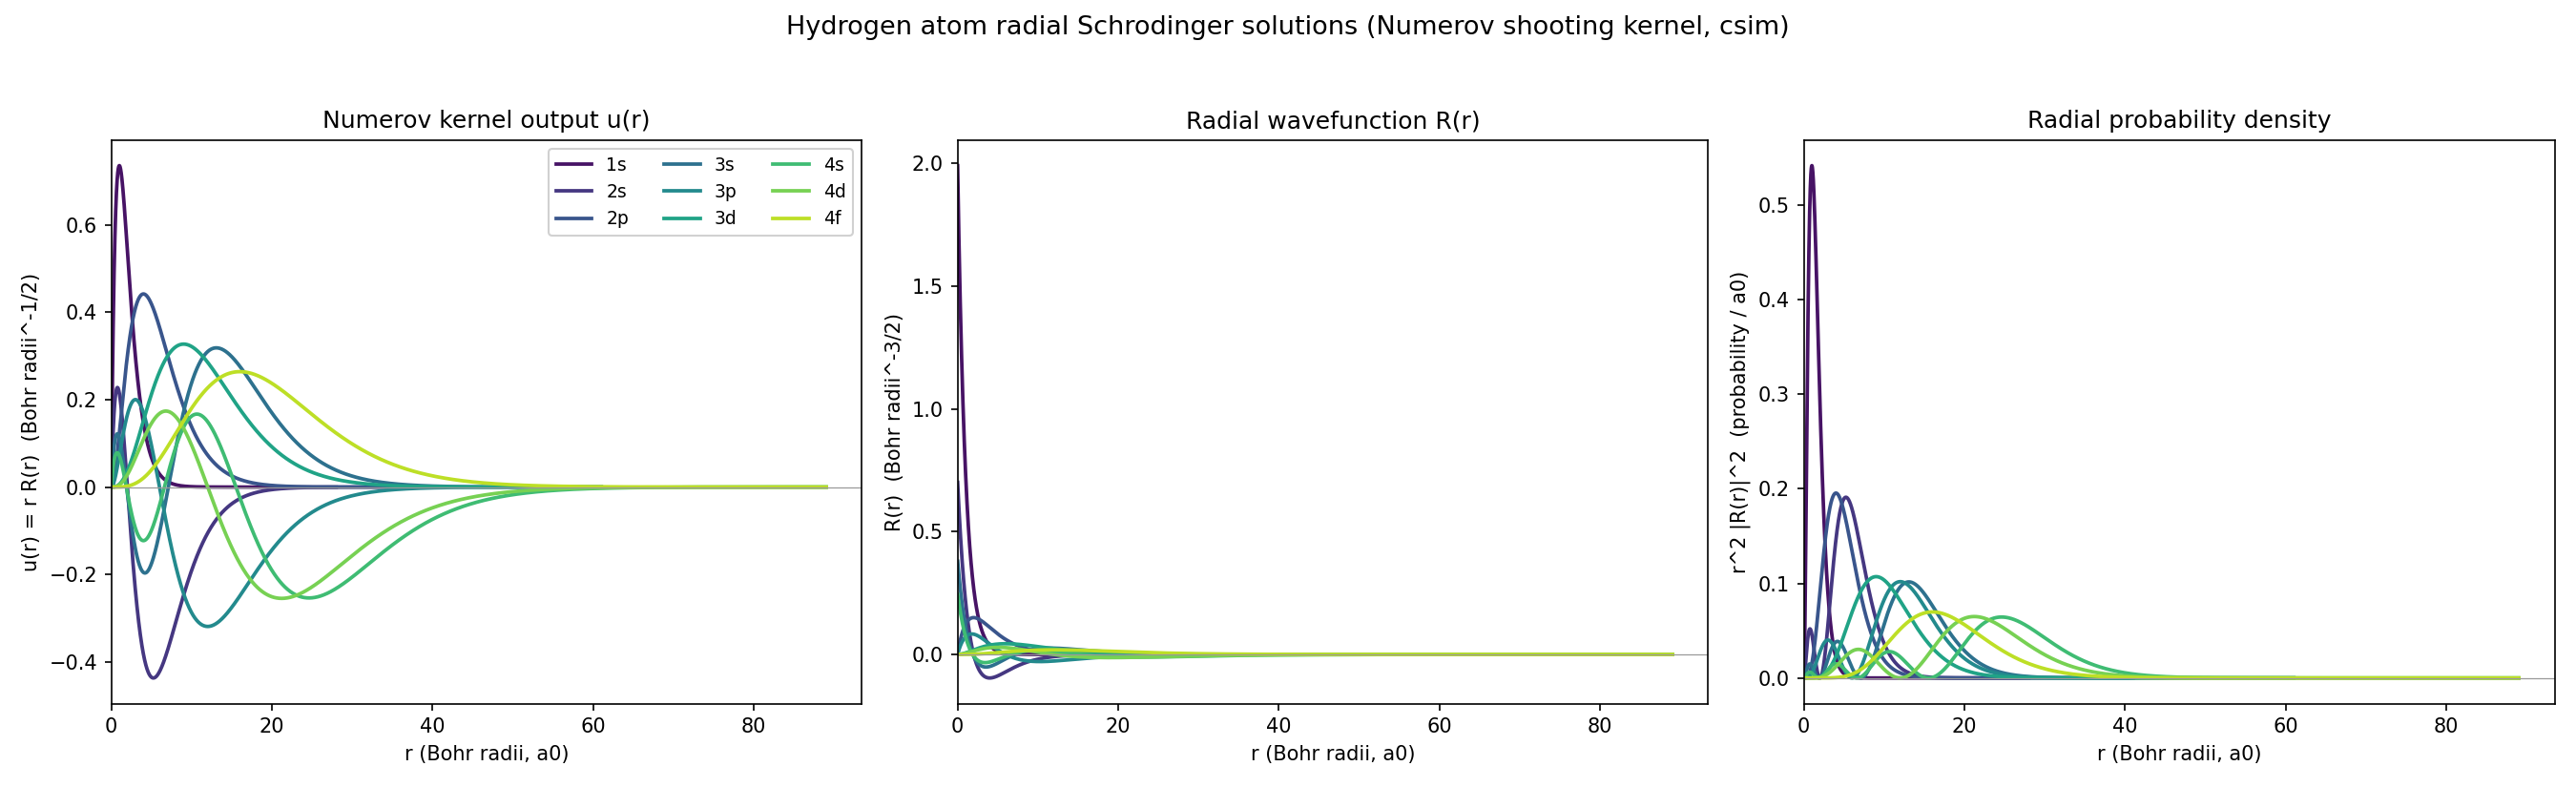
\includegraphics[width=\linewidth]{figures/hydrogen_radial_overview.png}
\caption{$u(r)$, $R(r)=u(r)/r$, and the radial probability density $r^2|R(r)|^2$ for all nine tested states, from the software co-simulation output.}
\label{fig:overview}
\end{figure}

\begin{figure}[t]
\centering
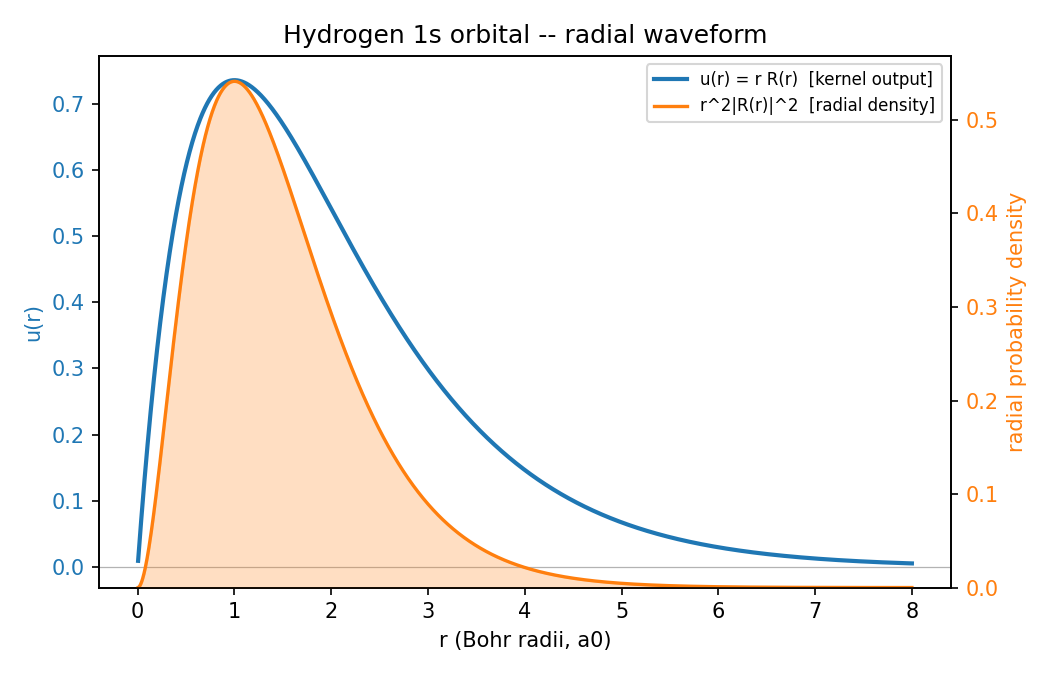
\includegraphics[width=0.48\linewidth]{figures/hydrogen_1s.png}\hfill
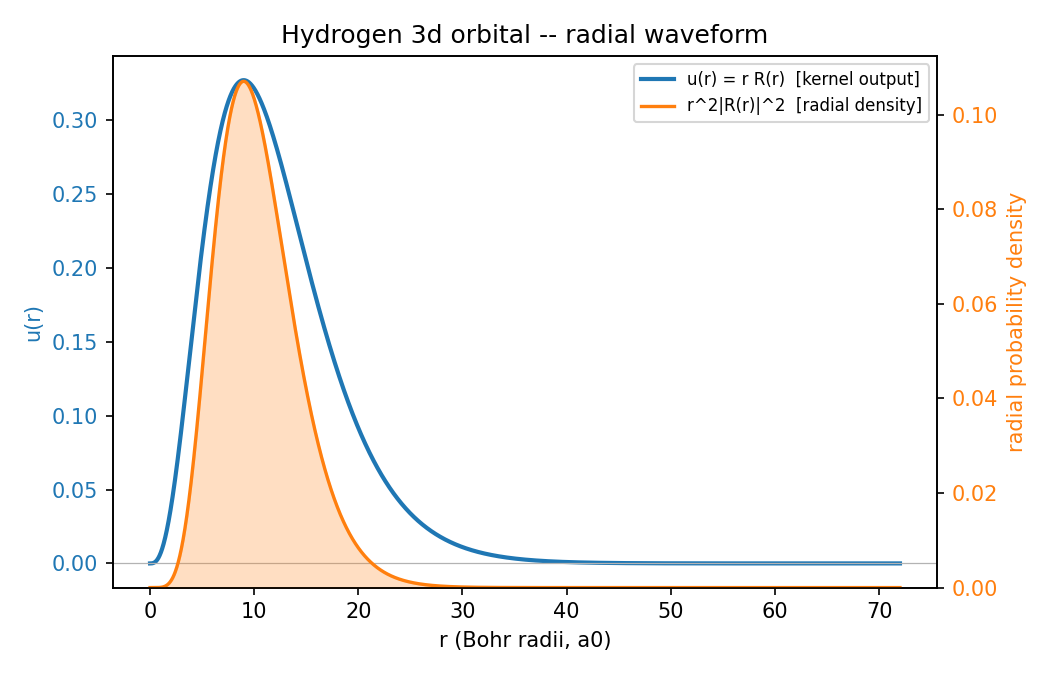
\includegraphics[width=0.48\linewidth]{figures/hydrogen_3d.png}
\caption{Individual-state radial waveform $u(r)$ (left axis) and radial probability density (right axis, filled) for $1s$ (left, the least numerically accurate state in Table~\ref{tab:accuracy}) and $3d$ (right, one of the most accurate).}
\label{fig:1s3d}
\end{figure}

% =============================================================================
\section{Discussion: what separates this from a hardware result}\label{sec:discussion}
% =============================================================================

We state plainly what this paper does and does not demonstrate, since the distinction matters for how the result should be used or cited.

\textbf{What is demonstrated.} A complete, HLS-pragma-annotated C++ kernel design, structured specifically to avoid dynamic control flow (Section~\ref{sec:kernel}), whose core numerical logic -- the Numerov recursion, the near-origin boundary condition, and the bisection eigenvalue search -- is verified correct to $10^{-6}$--$10^{-13}$ relative accuracy against exact closed-form quantum mechanics, by actually compiling and running the kernel's own source as a software co-simulation (Section~\ref{sec:results}).

\textbf{What is not (yet) demonstrated.} No FPGA synthesis, place-and-route, or hardware execution of this kernel has been performed. Concretely: (i) \texttt{build\_hydrogen/} contains only a \texttt{v++} build script and link configuration, no compiled \texttt{.xo}/\texttt{.xclbin} and no synthesis or implementation report of any kind, so we have no LUT/FF/DSP/BRAM utilization figures and no achieved clock frequency to report; (ii) the kernel's own build configuration sets a 225\,MHz clock target, but its accompanying comment explicitly labels this as borrowed from a different, already-built sibling kernel design and "not yet re-verified against a routed timing report for this kernel specifically," further noting that this kernel's double-precision-divide-heavy datapath is more divide-heavy than that sibling design and recommending a fallback to 200\,MHz "if place/route doesn't close" -- we repeat this caveat here rather than presenting 225\,MHz as an achieved or even a synthesis-confirmed figure; (iii) a Python XRT host driver for real-hardware execution exists in the repository, but its own docstring states it requires a pre-built \texttt{.xclbin} that does not currently exist, and it has correspondingly never been run against real hardware for this project.

\textbf{The identified risk that hardware bring-up must resolve.} The single most concrete open engineering question this design raises is whether the \texttt{II=1} pipelining target is achievable with a double-precision divide inside the Numerov update (Eq.~\eqref{eq:numerov}) on this device at a useful clock frequency -- double-precision division is typically one of the more resource- and latency-expensive operations HLS floating-point IP offers, and achieving initiation-interval-1 pipelining around it, across a fixed 8192-point inner loop repeated for 60 bisection iterations, is exactly the kind of claim that must be checked by an actual Vitis HLS \texttt{csynth} run and, ultimately, place-and-route -- neither of which has yet been done for this kernel.

% =============================================================================
\section{Conclusion and future work}\label{sec:conclusion}
% =============================================================================

This paper reported the design of an HLS kernel implementing a Numerov shooting-method solver for the hydrogen-atom radial Schr\"odinger equation, targeting an HBM-equipped Alveo U55C accelerator, built from fixed-trip-count loops specifically to be amenable to deterministic hardware pipelining, and validated -- by software co-simulation only -- to $10^{-6}$--$10^{-13}$ relative accuracy against exact closed-form quantum mechanics across nine bound states. We deliberately scoped this paper's claims to exactly what was verified: a correct numerical kernel design with a hardware-oriented interface, not yet a hardware result.

Future work, in priority order: (i) run Vitis HLS C-synthesis on the kernel and report the resulting resource-utilization and timing estimates, specifically checking whether the double-precision-divide-heavy Numerov update meets \texttt{II=1} at 225\,MHz or requires the documented 200\,MHz fallback (or a different precision strategy, e.g.\ a fixed-point or reduced-precision divide, as an alternative if timing does not close); (ii) complete the \texttt{v++} link and place-and-route flow to produce an actual \texttt{.xclbin} and a routed timing/utilization report; (iii) run the existing (but as-yet-unexercised) XRT host driver against that hardware and report measured latency, comparing it against the software co-simulation's arithmetic to confirm hardware/software equivalence, in the same spirit as the hardware/classical cross-validation methodology used in our companion surface-code study~\cite{ali_surface_code}; (iv) complete the missing $4p$ state in the test suite; and (v) extend the near-origin boundary condition beyond the two-term series of Eq.~\eqref{eq:bc} to reduce the $s$-state-specific error identified in Table~\ref{tab:accuracy}.

% =============================================================================
\backmatter

\section*{Declarations}

\textbf{Funding.} This work was carried out at the Centre for Development of Advanced Computing (C-DAC), Noida, India. \emph{[Author: insert specific grant/project number, if applicable, before submission.]}

\textbf{Conflict of interest.} The author declares no conflict of interest.

\textbf{Data and code availability.} The kernel source, software testbench, host-driver code, and the CSV/PNG data products reported in Section~\ref{sec:results} are available at \url{https://github.com/nasir26/fpga-mps-research}.

\textbf{Author contribution.} N.A.\ conceived the study, derived the numerical formulation, implemented the HLS kernel and testbench, ran the software co-simulation, and wrote the manuscript.

% =============================================================================
\begin{thebibliography}{99}

\bibitem{numerov1924} Numerov, B.V.: A method of extrapolation of perturbations. Mon. Not. R. Astron. Soc. \textbf{84}, 592--601 (1924)

\bibitem{cooley1961} Cooley, J.W.: An improved eigenvalue corrector formula for solving the Schr\"odinger equation for central fields. Math. Comp. \textbf{15}, 363--374 (1961)

\bibitem{thijssen2007} Thijssen, J.M.: Computational Physics, 2nd edn. Cambridge University Press, Cambridge (2007)

\bibitem{ali_rtl_statevector} Ali, N.: A Native RTL Quantum Statevector Simulator in FP64 on an HBM-Equipped FPGA. Submitted to J. Supercomput. (2026)

\bibitem{ali_30qubit_sim} Ali, N.: FPGA Based Quantum Circuit Simulator: Processing 30 Qubit Systems. Submitted to J. Supercomput. (2026)

\bibitem{ali_mps_engine} Ali, N.: Matrix Product State Engine for FPGA Quantum Circuit Simulation Beyond Five Hundred Qubits. Submitted to J. Supercomput. (2026)

\bibitem{ali_shor_steane_qec} Ali, N.: FPGA-Based Real-Time Quantum Error Correction for Shor and Steane Codes. Submitted to J. Supercomput. (2026)

\bibitem{ali_surface_code} Ali, N.: Hardware-in-the-Loop Verification of Distance-3 Surface-Code Quantum Memory on a 28-Qubit HBM-Accelerated FPGA Statevector Simulator. Submitted to J. Supercomput. (2026)

\bibitem{ali_statevector28} Ali, N.: From HBM Capacity to Measured Kernel Time: An Analytical Cost Model and CPU/GPU-Benchmarked Evaluation of a 28-Qubit-Capacity FPGA Statevector Simulator, with a ZX-Calculus Pre-Optimization Stage. Submitted to J. Supercomput. (2026)

\end{thebibliography}

\end{document}
